\documentclass[reprint,amsmath,amssymb,aps]{revtex4-2}

\usepackage{graphicx}% Include figure files
\usepackage{dcolumn}% Align table columns on decimal point
\usepackage{bm}% bold math
\usepackage{float}
\usepackage{amsmath}
\newcommand{\q}[1]{``#1''}

\usepackage{xcolor}

%comment from Daniel:
\newcommand{\dms}[1]{{\color{blue} #1}}

\DeclareMathOperator\arctanh{arctanh}
\DeclareMathOperator\arccosh{arccosh}

\begin{document}

%Title of paper
\title{Hierarchical structure of the energy landscape in the Voronoi model of dense tissue}

\author{Diogo E. P. Pinto$^{1,2}$, Daniel M. Sussman$^{3}$, Margarida M. Telo da Gama$^{1,2}$ and Nuno A. M. Ara\'{u}jo$^{1,2}$}

\affiliation{$^{1}$ Centro de Física Teórica e Computacional, Faculdade de Ciências, Universidade de Lisboa, 1749-016 Lisboa, Portugal. \\ $^{2}$ Departamento de Física, Faculdade de Ciências, Universidade de Lisboa, 1749-016 Lisboa, Portugal.  \\ $^{3}$ Department of Physics, Emory University, Atlanta, GA, USA}

\begin{abstract}
The Voronoi model is a popular tool for studying confluent living tissues. It exhibits an anomalous glassy behavior even at very low temperatures or weak active self-propulsion, and at zero temperature the model is a disordered solid with no evidence of a rigidity transition. Here we investigate the properties of the energy landscape in this limit. We find two disordered solid phases that have similar structural features but that differ in the ultrametricity of their energy landscapes; the crossover between these two states shares phenomenological properties with a Gardner transition. We further highlight the importance of the precise choice of metric when calculating the distance between configurations for detecting hierarchical arrangements of basins in the energy landscape.
\end{abstract}

%\maketitle must follow title, authors, abstract, \pacs, and \keywords
\maketitle

\begin{figure*}[t]
	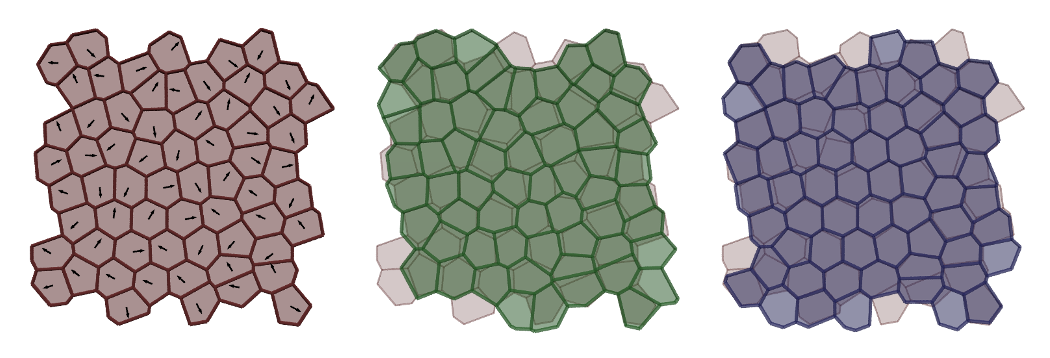
\includegraphics{fig1.eps}
	\caption{\label{model} Representation of the perturbation protocol. On the left is represented the original minimized configuration (red) with the perturbation vectors in the center of each cell. In the middle is the original minimized configuration (red) and the perturbed one (green). On the right is the original minimized configuration (red) and the one minimized after the perturbation (blue).}
\end{figure*}

Understanding the collective behavior of cells in biological tissues has become one of the major interdisciplinary challenges of recent years, with applications ranging from wound healing to cancer treatment~\cite{Ghosh2007, Gov2009, Park2015, Tambe2011, PerezGonzalez2018, Sunyer2016}. Both experimental and theoretical efforts have been crucial in understanding the properties of these tissues and the mechanisms by which tissue properties are regulated, for example in the way that tissues can transition from rigid to flexible as the properties of individual cells are regulated~\cite{Angelini2011, Garcia2015, Park2015, Schotz2013, mongera2018fluid,Grosser2021,devany2021cell}. Rigidity transitions are also seen in particulate systems, such as granular materials and colloidal suspensions, in which changes in particle density and temperature can lead to disordered materials in a kinetically arrested jammed or glassy state~\cite{Binder1986, Berthier2011, Janssen2019}. In living tissues, the nature and properties of the rigid states are still under debate~\cite{Angelini2011, Garcia2015, Park2015, Schotz2013}, owing both to the explicitly non-equilibrium nature of cellular motion and the many-body interactions found in confluent tissue~\cite{Szavo2006}. These differences raise several challenges to the generalization of ideas and methods developed in the context well-studied particulate matter~\cite{Merkel2018, Merkel2019, Angelini2011, Tambe2011, PerezGonzalez2018}.

Several models have been proposed to understand the collective behavior of cellular systems, from single particle descriptions to density field models~\cite{Bi2014, Bi2015, Farhadifar2007, Fletcher2014, Camley2017, Kabla2012}. The Voronoi model represents a confluent tissue as a space filling polygnal tiling, where each positional degree of freedom corresponds to a cell whose shape is obtained by an instantaneous Voronoi tessellation~\cite{Bi2016,Kaliman2016, Sussman2018a}. The dynamics is controlled by an energy functional that is quadratic in the area and perimeter of each cell (described in more detail below), and the mechanical properties of the tissue can be either solid-like or fluid-like depending on the temperature and a shape parameter, $p_0$, which quantifies the target shape of the individual cells~\cite{Bi2016}.

At zero temperature (or in the absence of cellular activity) it has been argued that the Voronoi model possesses a finite shear modulus over its entire range of model parameters~\cite{Sussman2018}. This is in sharp contrast with particulate systems, in which a zero-temperature rigidity transition can be observed by changing the system density~\cite{Parisi2010, Goodrich2012, Charbonneau2017, Baule2018}. The particulate jamming transition is typically interpreted in the context of constraint counting, in which the transition occurs when the number of independent particle-particle contacts equals the number of degrees of freedom~\cite{Lubensky2015,franz2019critical}. As described below, in the 2D Voronoi model the energy function is always at this point of marginal stability~\cite{Sussman2018}, and thus an analysis based only on the balance between constraints and degrees of freedom is insufficient. It has been proposed instead that energetic rigidity, in which not only simple constraints but also residual stresses can play a controlling role~\cite{Merkel2018, Merkel2019,Yan2019, Damavandi2021}, is a better framework for understanding Voronoi model rigidity in the athermal limit~\cite{Damavandi2021}.

Here we explore this unusual athermal regime of the Voronoi model and show that, even in the absence of a zero-temperature rigidity transition, there is nevertheless a profound change in the statistics of the energy landscape in different parts of model parameter space. We find the evidence for a transition to an ultrametric, hierarchical arrangement of basins in the energy landscape, suggesting two different phases of disordered solid~\cite{Charbonneau2015, Liao2019, Artiaco2020, Dennis2020}. The ultrametric state is characterized by energy minima forming a tree-like structure in phase space where minima within a given sub-basin are much closer to one another than they are to minima in any other sub-basin~\cite{Parisi2010, Charbonneau2017}. This is consistent with a Gardner phenomenology~\cite{Parisi2010, Charbonneau2017}; the phenomenological properties of this phase have been studied in multiple experimental and computational systems~\cite{Charbonneau2015,seguin2016experimental,scalliet2017absence,Liao2019, Artiaco2020, Dennis2020}.

We model the confluent tissue as a monolayer of $N$ cells~\cite{Bi2016,Bi2014,Bi2015} in a square domain of side-length $L$ with periodic boundary conditions. Each cell $i$ is represented by its center $\textbf{r}_i$ with a shape given by an instantaneous Voronoi tessellation of the space. We choose the unit of length to be given by the square root of the average area of all the cells. We can then write a dimensionless version of the contribution of each cell to the energy functional as~\cite{Farhadifar2007,Fletcher2014,Merkel2018,Teomy2018a}
\begin{equation}\label{eq::en_func_reduced}
	%
	e_i=k_A(a_i-1)^2+(p_i-p_{0})^2.
	%
\end{equation}
Here $a_i$ and $p_i$ are the dimensionless area and perimeter of cell $i$, $p_0$ is the target perimeter, and $k_A$ represents the ratio between the relative stiffness of the area and perimeter elasticity terms for the cell. Biologically, the first term models cellular incompressibility and the resistance of the cellular monolayer to height fluctuations; the second term models the competition between active contractility of the actomyosin subcellular cortex and the effective cell membrane tension due to cell-cell adhesion and cortical tension.

\begin{figure*}[t]
	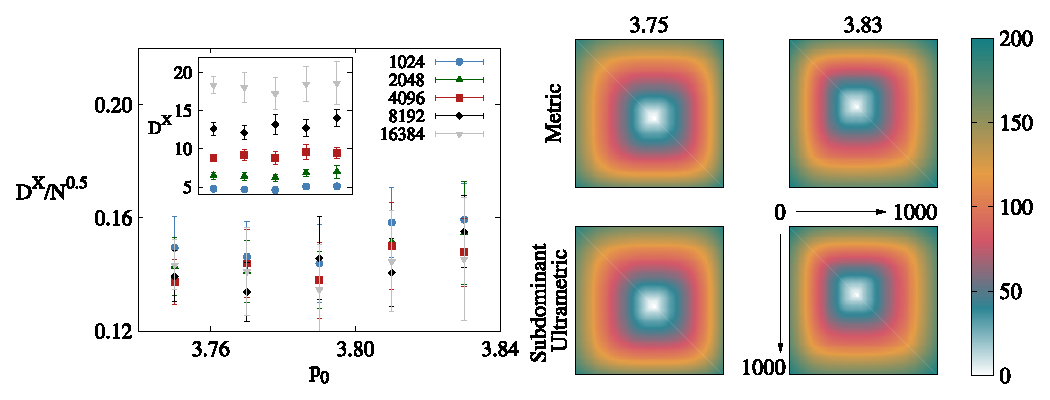
\includegraphics{fig2.eps}
	\caption{\label{PosMetric} (Left) The normalized generalized distance to ultrametricity as measured using the contact vector metric, $D^X/\sqrt{N}$, as a function of  $p_0$, for $N=1024, 2048, 4096, 8192, 16384$. The inset shows the same results without the scaling. (Right) A schematic representation of the distances between minima according to the contact metric, $d^X(a,b)$, and the subdominant ultrametric constructed from it using a minimum spanning tree~\cite{Kruskal1956, Rammal1985}. Matrices corresponding to $N=4096$ and $p_0 = 3.75,\ 3.83$ are shown, where the different distances are grouped using a single-linkage clustering algorithm which clusters the minima sequentially by distance. All results are averages of 10 initial configurations subject to 100 perturbations and minimizations each.}
\end{figure*}

For each set of parameters, we start with $N$ cells distributed at random positions. The configuration is then minimized using the FIRE algorithm~\cite{Bitzek2006}, which we halt when the maximum net force on each cell is less than $10^{-12}$. Due to numerical constraints, we consider $p_0\leqslant3.85$, since it has been shown for athermal systems that, above this value, configurations with multi-fold vertices are obtained which lead to numerical instabilities in the minimization protocol~\cite{Sussman2018}. Further details of the simulations can be found in the \textit{Supplemental Material}.


To probe the structure of the energy landscape, we start from an initial configuration that corresponds to a local minimum and perturb it to find new stable configurations. In our primary perturbation protocol, we displace the position of each cell according to the vector $\overrightarrow{P}_{\varepsilon}=[X_0, X_1,\ldots, X_{2N-1}]$, where $N$ is the number of cells, $X_{2i}=\varepsilon\cos(\theta_i)$ is the perturbation to cell $i$ along the $x$-axis, $X_{2i+1}=\varepsilon\sin(\theta_i)$ is the one along the $y$-axis, and $\theta_i$ is a random angle uniformly distributed between $0$ and $2\pi$. We considered a random length $\varepsilon$ drawn from a uniform distribution between $0$ and $\varepsilon_{max}$, to guarantee the possibility of visiting minima in the same and different top-level basins. The norm of the perturbation vector is $|\overrightarrow{P}_{\varepsilon}|=P_{\varepsilon}=\varepsilon\sqrt{N}$. After the perturbation, we subtract the global translation of the tissue, and then let the tissue relax to a new minimum. An example of this process is shown in Fig.~\ref{model}; details of alternate ``perturb-and-minimize'' schemes can be found in the \textit{Supplemental Material}, where we show that our results are not qualitatively sensitive to these details.


We will be exploring different metrics to characterize distances between minima in the energy landscape. To begin quantifying these distances we first consider the contact metric (denoted by the superscripted $X$) discussed in Refs.~\cite{Dennis2020, Liao2019, Artiaco2020},
\begin{equation}\label{metric}
	d^X(a,b)=\sqrt{\sum_{ij}(\vec{C}^{a}_{ij}-\vec{C}^{b}_{ij})^2},
\end{equation}
where $d^X(a,b)$ is the distance between configuration $a$ and $b$, and $\vec{C}^{a}_{ij}$ is the 2D contact vector between two cells, where each component $C^{a}_{ij,x}=x_i^a-x_j^a$ is the distance along the respective axis between cells $i$ and $j$ if those cells share and edge, and $\vec{C}^{a}_{ij}=\vec{0}$ otherwise. In the \textit{Supplemental Material}, we show how the normalized distance to the original minimum, $d^X_N(a,b)=d^X(a,b)/\sqrt{|a| |b|}$, where the norm of a configuration corresponds to $|a|=d^X(a,0)$, scales with the number of cells and the norm of the perturbation vector. We observe that $d^X(a,b)\sim\sqrt{N}$ and choose $\varepsilon_{max}=0.5\sqrt{N}$ for all $p_{0}$, which is large enough so that the perturbed configuration does not always relax to the initial minimum but small enough that nearby minima are accessible.


Figure \ref{PosMetric} shows matrices where the color corresponds to the distance between minima, for all pairs of minima found for $p_0=3.75$ and $3.83$. These matrices were constructed for $10^3$ minima obtained for a tissue of $4096$ cells. Each element of the matrix corresponds to the distance between two minima, $a$ and $b$, given by Eq.~\eqref{metric}. The distances are all sorted using the single-linkage clustering algorithm on the metric of the fully minimized systems, which groups them sequentially based on their relative distance~\cite{Murtagh1983}. The colors represent different distances. In white are the minima that are closest to each other. We can see groups of minima that are all at this minimum distance, forming a white region that corresponds to sub-basins. The matrices do not show any substantial visual change with $p_0$.

\begin{figure*}[t!]
	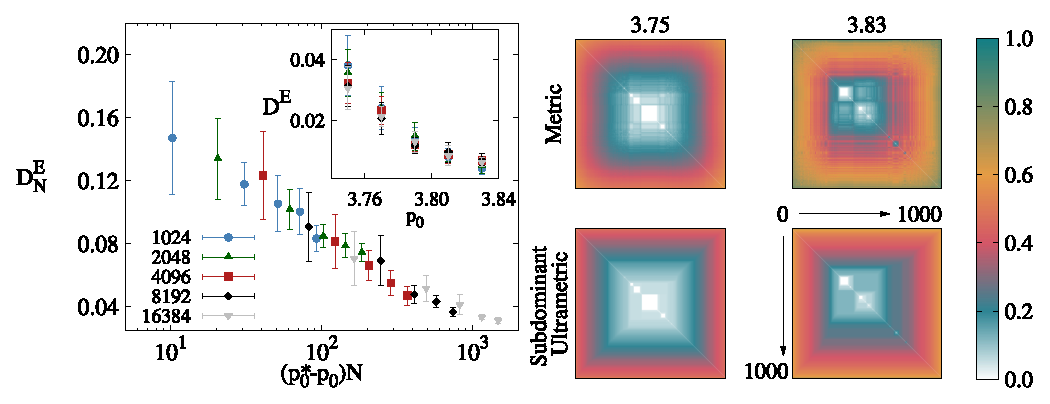
\includegraphics{fig3.eps}
	\caption{\label{EnergyMetric} (Left) The normalized generalized distance to ultrametricity as measured using the normalized energy metric, $D^E_N$,  as a function of $(p_0^*-p_0)N^{0.4}$, for $N=1024, 2048, 4096, 8192, 16384$ and $p_0^*=3.89\pm 0.01$. The inset shows the generalized distance to ultrametricity, $D^E$, calculated using the energy metric, $d^E(a,b)$, as a function of $p_0$, for the same $N$. (Right) Schematic matrix representation of the distances between minima according to the normalized energy metric, $d_N^E(a,b)$, and its subdominant ultrametric, as in Fig.~\ref{PosMetric}. Matrices are shown for $p_0=3.75,\ 3.83$ and $N=4096$. All results are averages of 10 initial configurations subject to 100 perturbations and minimizations each.
	}
\end{figure*}

A Gardner phase is characterized by an ultrametric phase space consisting of a tree-like structure, where minima within a given sub-basin are all much closer to one another than to minima in any other sub-basin. This property is codified by an ultrametric inequality,
\begin{equation}
\label{ultraIneq}
d^X(a,c)\leq \text{max}[d^X(a,b) , d^X(b,c)] ,
\end{equation}
where $a, b$ and $c$ are three different configurations in phase space and $d^X(a,b)$ the distance, given by Eq.~\eqref{metric}, between them. To verify if the properties of the tissue are consistent with a Gardner phase, we compute how close the metric is to being an ultrametric. To do so, we first find the subdominant ultrametric, $d^<(a,b)$, i.e., the ultrametric that is closest to $d^X(a,b)$ itself. The subdominant ultrametric can be found by first computing the distances in the minimum spanning tree of the space of minima. Then, for each pair of minima $a$ and $b$, we compute the path between them in the minimum spanning tree and define $d^<(a,b)$ as the largest distance between two neighboring minima along the path~\citep{Rammal1985}. The corresponding matrices are shown in Fig.~\ref{PosMetric}.

Having found $d^<(a,b)$, we finally calculate the generalized distance between the metric and the subdominant ultrametric using
\begin{equation}\label{genDist}
	D^X=\sqrt{\langle (d^X(a,b)-d^<(a,b))^2 \rangle},
\end{equation}
where $\langle \cdot \rangle$ denotes the average over all configuration pairs $a$ and $b$. If $D^X=0$ then the energy landscape is ultrametric, while $D^X>0$ quantifies how far it is from ultrametricity. In the inset of Fig.~\ref{PosMetric}, we show that $D^X$ increases only slightly with $p_0$, but more importantly it also depends strongly on  $N$. In the main plot we re-scale $D^X/\sqrt{N}$ and obtain reasonable collapse of the data. Since the typical distance between minima and the distance to ultrametricity both scale with $\sqrt{N}$, the space with this contact metric is not ultrametric in the thermodynamic limit~\cite{Dennis2020}.


Using distances based on the contact vectors suggests that the landscape of the Voronoi model is not ultrametric, but does the choice of metric itself influence this result? We note that in the Voronoi model, the contact network of the tissue does not change significantly even as the tissue rigidity changes substantially~\cite{Damavandi2021, Merkel2019}. We further note that the energy functional in Eq.~\eqref{eq::en_func_reduced} is a simple collection of harmonic springs, but in a coordinate basis of shape space rather than in the positional basis of the degrees of freedom generating the shapes. This suggests a different metric might be more appropriate, and in this context we propose one based on the contribution of each cell $i$ to the total energy of the tissue, $E_i$. We take the same form for the metric as Eq.~\eqref{metric}, but where $\vec{C}^a_{ij}\rightarrow C^a_{ij}=E^a_i-E^a_j$, if $i$ and $j$ are neighbors and zero otherwise. We call this metric the ``energy metric'', $d^E(a,b)$. We adopt the same perturb-and-minimize protocol as before, using  $\varepsilon_{max}=0.1\sqrt{N}$ for all $p_{0}$. As such, we keep biasing the perturbations to nearby minima in the new metric, otherwise more simulations would be needed to probe the same volume of configuration space. In the \textit{Supplemental Material} we show that the results using the contact metric remain qualitatively the same using the new  $\varepsilon_{max}$. Just like the contact metric, the energy metric scales with system size, $d^E(a,b)\sim\sqrt{N}$, since it depends on the total number of cell-cell contacts.  We observe in the inset of Fig. \ref{EnergyMetric} that, for the energy metric, the distance to ultrametricity ($D^E$) does not scale with $N$ and decreases with $p_0$ (inset of Fig.~\ref{EnergyMetric}). Since the distance between minima scales as $d^E(a,b)\sim\sqrt{N}$, while the generalized distance does not depend on the system size, this suggests that the system does, in fact, become ultrametric in the thermodynamic limit: $D^E/d^E(a,b)\sim 1/\sqrt{N}$.

In the case of the contact metric the calculated values are already normalized since we increase the box size with $N$, while the typical cell size is fixed. In the case of the energy metric this is no longer the case. Thus, to properly compare system properties at different $p_0$ values (since $\langle E_i\rangle$ varies with $p_0$), we also consider a normalized version of the energy metric: $d^E_N(a,b)=d^E(a,b)/\sqrt{|a| |b|}$, for which the typical distance between configurations does not depend on either $p_0$ or $N$. Figure \ref{EnergyMetric} shows the schematic representation of the normalized energy metric, $d_N^E(a,b)$, and its subdominant ultrametric. From this representation, we can already observe changes in the structure of the energy landscape structure. As $p_0$ increases, the color gradient is less smooth and the boxes corresponding to the different sub-basin become sharper. Furthermore, it is also observed that more minima fall into the same sub-basin. These properties suggest that, when the value of $p_0$ decreases, the structure of the energy landscape becomes more hierarchical~\citep{Dennis2020}.

We also compute the generalized distance to ultrametricity when using $d_N^E$. Again we see that ultrametricity is approached with increasing system size. Furthermore, with the scaling shown in the main panel of  Fig.~\ref{EnergyMetric} we can collapse the different curves. Recent work in particulate systems has interpreted similar scaling as a distance to jamming~\cite{Dennis2020, Goodrich2012}. This suggests not only that the Voronoi model has an ultrametric structure in the thermodynamic limit, but that there may be a transition between two different solid phases. Previously, it was shown that the athermal Voronoi model did not have a rigidity transition~\cite{Sussman2018}. Nevertheless, we show that there is a clear difference between the energy landscape for low and high $p_0$: at low $p_0$ the glass state is characterized by large residual stresses and an ultrametric energy landscape, and at high $p_0$ the energy landscape is not. We find that the change in the structure of the energy landscape occurs for preferred shape parameters between $p_0=3.75-3.83$, which is close to the where the zero-temperature shear modulus changes markedly~\cite{Sussman2018} and where dynamics at finite temperature has a change in character~\cite{Bi2016, Sussman2018a,Li2021}.

\begin{figure*}[t!]
	\includegraphics{fig4.eps}
	\caption{\label{EnergyKAMetric} (Left) A plot similar to Fig.~\ref{EnergyMetric} but for $k_A=0$, highlighting the similar scaling in the two cases. Here, we use $p_0^*=3.798$. (Right) Schematic representations of the normalized energy metrics, $d_N^E(a,b)$, of systems with size $N=4096$, $k_A={0,0.01,1,100}$ and $p_0={3.75, 3.77, 3.83}$. For $k_A=0$ and $p_0=3.83$ the metrics only show one color since $E_i-E_f\approx 0$ and thus the normalized metric distance diverges. All results are averages of 10 initial configurations subject to 100 perturbations and minimizations each.
	}
\end{figure*}


As $p_0$ increases, fewer sub-basins are found inside each basin (as represented by the different unconnected clusters in Fig.~\ref{EnergyMetric}), suggesting that the energy landscape flattens out. Another way of exploring this flattening of the energy landscape is by studying the behavior of the model as the relative area modulus $k_A$ is varied. In the limit $k_A=0$ the Voronoi model is no longer marginally constrained, and it acquires a residual-stress-based rigidity transition as a function of $p_0$ at $T=0$~\cite{Sussman2018}. As shown in Fig.~\ref{EnergyKAMetric}, for $p_0<3.79$ we find that the tissue is both rigid and the energy landscape is ultrametric. For slightly larger $p_0$ the energy landscape deviates from ultrametricity and its variance increases significantly. In this regime, the energy landscape consists of a mixture of hierarchical basins and several nearly flat basins and so, in many cases, small perturbations will not drive the system to a different minimum. Due to finite size effects it is difficult to asses if a new solid phase exists. In the \textit{Supplemental Material} we use a simple technique to estimate the transition from the solid to the fluid phase. Using the fraction of configurations with zero energy we estimate a transition point around $p_0^*=3.8022\pm0.0001$, while in Fig.~\ref{EnergyKAMetric} $p_0^*=3.798\pm 0.001$ is a more appropriate value to collapse the data. More simulations would be needed to properly conclude if a new solid phase at $k_A=0$ exists before the fluid phase, or if what we observe are only finite size effects and both transition points actually coincide. For $p_0>3.8$ the energy landscape is flat, characteristic of a fluid-like tissue. For any $k_A>0$, different energy minima are found for all $p_0$, consistent with previous work showing a finite shear modulus for all the range of model parameters studied~\cite{Sussman2018}. The qualitative properties of these phases can be seen in the matrices shown in Fig.~\ref{EnergyKAMetric}. Although we have not explored the thermal case, recent studies with the thermal 2D Voronoi model also suggest a change in the energy landscape close to $p_0\approx3.81$, where there is an emergence of a fractal-like energy landscape and cells become virtually free to diffuse in specific phase space directions up to a small distance~\cite{Li2021}.

In summary, we have found indications of a hierarchical structure of the energy landscape in a model of dense biological tissue whose zero-temperature rigidity is quite different from that of constraint-based particulate systems. Strikingly, we find that the choice of metric to characterize distance between minima is crucially: defining distance based on changes in neighboring contact vectors vs contributions to the energy give \emph{qualitatively} different interpretations to the structure of the energy landscape. In particulate systems the contact vectors directly enter the relevant energy functional -- i.e., the energy of a soft harmonic repulsion or a Lennard-Jones interaction is a simple function of the contact vector between interacting particles. In Voronoi models the energy cannot be decomposed into independent pairwise contributions, which we speculate is the reason that choosing a distance metric based on the total energy associated with each degree of freedom is able to uncover the hierarchical structure of the landscape. We further speculate that this may point more generally to the importance of the choice of metric for systems in which many-body interactions dominate over pairwise ones. An avenue for future research could be relating these tissue-like systems to particulate ones, such as soft or hard spheres~\cite{Liao2019, Dennis2020}. This could be done by establishing the relation between the effects of $p_0$ in the Voronoi model and pressure in particulate systems. Since both exhibit an ultrametric landscape, this could allow for a generalization of glassy physics outside of particulate systems and glass-forming materials~\cite{Berthier2011, Parisi2010, Janssen2019}.

%------------------------------------
%------------------------------------
%------------------------------------

\section{Acknowledgments}

The authors acknowledge financial support from the Portuguese Foundation for
Science and Technology (FCT) under Contracts no. PTDC/FIS-MAC/28146/2017
(LISBOA-01-0145-FEDER-028146), UIDB/00618/2020, UIDP/00618/2020 and
SFRH/BD/131158/2017.

%------------------------------------
%------------------------------------
%------------------------------------

% \section{Supplemental Material}
%
% \subsection{Simulation details}
%
% To simulate the tissue we use cellGPU \cite{Sussman2017} and initialize $N$ cells distributed randomly in a square periodic box of linear size $\sqrt{N}$ in units of $\sqrt{\bar{A}}$. We consider a monodispersed system with $\bar{A}=1$.
%
% \begin{figure}[b]
% 	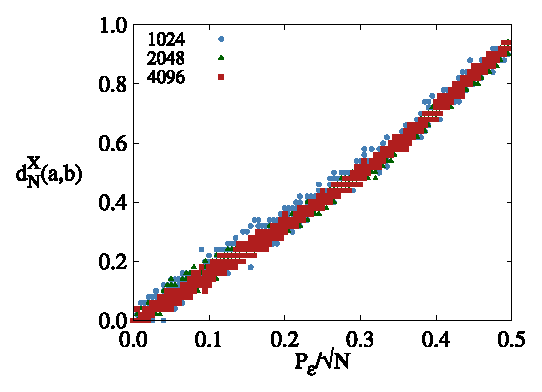
\includegraphics{fig5.eps}
% 	\caption{\label{CM}Scatter plot of the distribution of normalized metric distance to the original minimum for different norms of the perturbation vector, using the contact metric. The metric distance defined in Eq.~\eqref{metric} is normalized by $\sqrt{|a| |b|}$, where $|a|=d(a,0)$. For $p_0=3.81$, all sizes collapse into the same curve when using this scaling, thus we choose $\varepsilon_{max}=0.5\sqrt{N}$.}
% \end{figure}
%
% After initialization, the tissue is relaxed using a FIRE minimization algorithm \cite{Bitzek2006}. This relaxation algorithm moves the cell centers at each step in order to minimize the energy, following the functional form given in Eq.~\eqref{eq::en_func_reduced}. To do so, it uses the standard Molecular dynamics equations (with Euler integration) and two adaptive quantities, the time-step $\Delta t$ and $\alpha$, the later to adjust the integration step and the former to control the velocities. During the relaxation, when a \textit{uphill} in the energy landscape is found both change in order to minimize the amount of time spent there and then increase again when a \textit{downhill} appears. For our simulations, we have chosen $\Delta t_{min}=0.001$, $\Delta t_{max}=0.1$ and $\alpha_{start}=0.99$. We have tested other values and have found that they do not affect substantially the minimization procedure. Thus, they were kept the same for all cases. The minimization is halted once the maximum force on all cells is less than $10^{-12}$ in natural units (see previous section).
%
% \begin{figure}[t]
% 	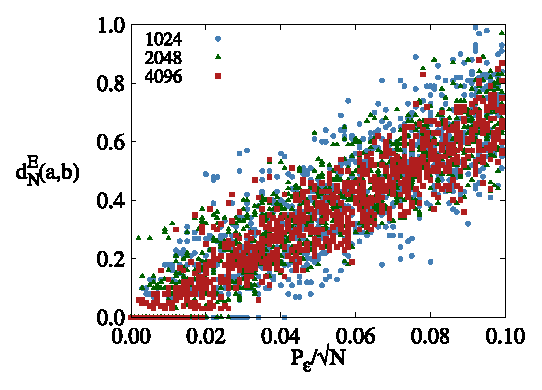
\includegraphics{fig6.eps}
% 	\caption{\label{EM}Scatter plot of the distribution of normalized metric distance to the original minimum for different norms of the perturbation vector, using the energy metric. The metric distance defined in Eq.~\eqref{metric} is normalized by $\sqrt{|a| |b|}$, where $|a|=d(a,0)$. For $p_0=3.81$, all sizes collapse into the same curve when using this scaling, thus we choose $\varepsilon_{max}=0.1\sqrt{N}$.}
% \end{figure}
%
% Figure \ref{CM} shows how the normalized distance to the original minimum, using the contact metric, scales with the norm of the perturbation vector applied, computed after subtracting the global translation, where $|a|=\sqrt{\sum_{ij}(C^{ij}_a)^2}$ corresponds to $d^X(a,b)$ for which $C^{ij}_b=0$. Here, $a$ was fixed and corresponds to the initial configuration, while $b$ is the minimum after the perturbation. We observe that the distance to the original minimum scales approximately linearly with the norm of the perturbation. Furthermore, as in ref.~\cite{Dennis2020}, by rescaling the perturbation by $\sqrt{N}$ we collapse the curves for different system sizes. To properly parameterize $\varepsilon_{max}$, we need to choose a value that is large enough so that the perturbed configuration does not relax to the initial minimum but small enough so that we can guarantee that, in principle, any minimum that has some structural resemblance (a normalized distance value smaller than one) to the unperturbed one is accessible. We choose $\varepsilon_{max}=0.5\sqrt{N}$ for all $p_{0}$, based on these results.
%
% By doing the same analysis using the energy metric we get Fig.~\ref{EM}. From the same reasoning as stated above, we choose $\varepsilon_{max}=0.1\sqrt{N}$ for all $p_{0}$, based on these results.
%
%
% \subsection{Contact metric}
%
% If we use the same perturbation as in the energy metric ($\varepsilon_{max}=0.1\sqrt{N}$) we are only able to reach maximum distances of $d^X(a,b)\approx0.23$. By making the same analysis as in the main text, we find the results in Fig.~\ref{CM_SP_D}. From these matrices it is possible to see the structure of the basins more clearly but the results remain qualitatively the same.
%
% \begin{figure*}[t]
% 	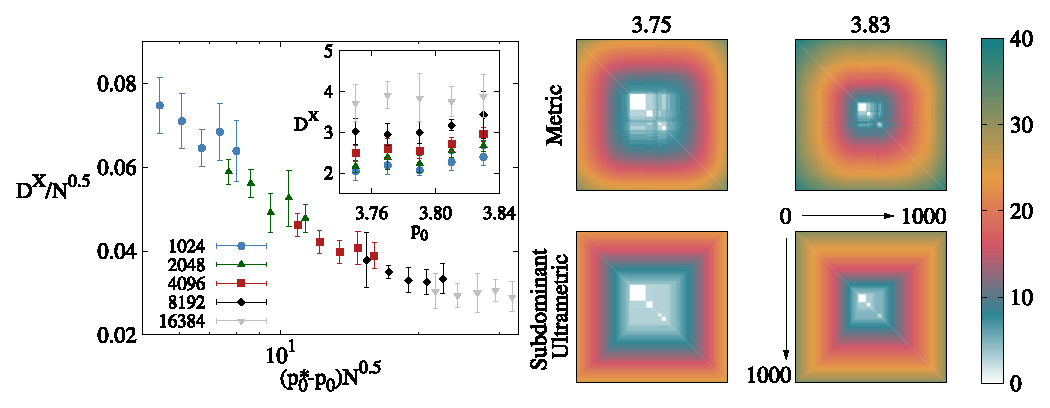
\includegraphics{fig7.eps}
% 	\caption{\label{CM_SP_D} On the right is a schematic representation of the distances between minima according to the contact metric and its corresponding subdominant ultrametric. We show the matrices for $p_0=3.75, 3.83$, with $1000$ different minima and $N=4096$. The different distances are grouped using a single-linkage clustering algorithm. On the left is a plot of the normalized distance to ultrametricity (Eq.~\eqref{genDist}) as a function of $(p_0^*-p_0)$, where we have chosen $p_0^*=3.92\pm 0.01$, for $N=1024, 2048, 4096, 8192, 16384$. The inset shows the same results without this scaling. These results were averaged using $10$ different configurations with each being perturbed and re-minimized $100$ different times.}
% \end{figure*}
%
% \subsection{$k_A\neq1$ cases}
%
% Here we explore the changes to the energy landscape for different $k_A$. We explore the values $k_A=\{0,10^{-2},10^0,10^2\}$. For finite $k_A$ a transition to the fluid-like state never occurs and the system is always rigid. Nonetheless, features of a transition between rigid states are still present for all $k_A$.
%
% In Fig.~\ref{EM_KA} we can observe how the different $k_A$ change the hierarchy of the energy landscape, using the generalized distance to ultrametricity (Eq.~\eqref{genDist}). We can find that qualitatively the results are similar for the different $k_A$, especially $k_A=1$ and $k_A=100$. For $k_A=0.01$, the variance of $D_N^E$ increases significantly around $p_0=3.81$, while for the others this is not as pronounced. This is due to the fact that the energy landscape partially flattens and there is a coexistence between basins with multiple sub-basins and basins which are almost flat where any (small) perturbation always leads to the same minimum.
%
% Although the variance seems to reduce significantly for $p_0=3.83$, this might be due to the presence of multi-fold vertices. Since we are not able to take these vertices into account in our simulations, we have to discard them. This leaves a smaller pool of minima to sample which might lead to smaller fluctuations.
%
% \begin{figure}[b]
% 	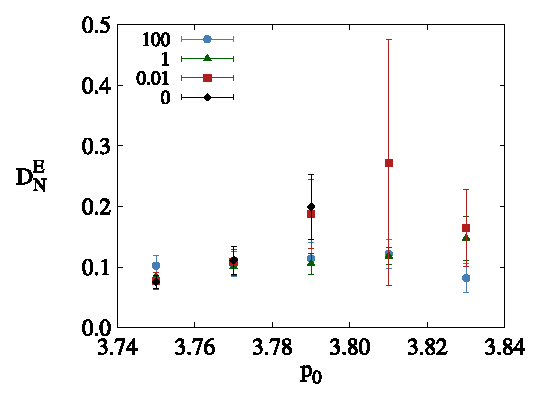
\includegraphics{fig8.eps}
% 	\caption{\label{EM_KA} Generalized distance to ultrametricity, for the normalized energy metric, $D^E_N$, as a function of $p_0$. Here we make a comparison between different $k_A$, using system with size $N=1024$. These results were averaged over $10$ different systems with each being perturbed and re-minimized $100$ different times.}
% \end{figure}
%
% \subsection{Energy metric with similar distance distributions}
%
% One thing to note is that there is a dependence of the distances explored with $p_0$ when using the energy metric, with increasing $p_0$ leading to larger distances. Here, we change $\varepsilon_{max}$ for different $p_0$, in such a way that similar ranges of normalized energy metric distance are found. In Fig.~\ref{EM_P0_D} we show how the generalized distance to ultrametricity, $D^E_N$, changes as a function of $p_0$, using a constant $\varepsilon_{max}$ and a variable one that depends on $p_0$. We can observe that although the values change slightly the qualitative description of the results remains the same as the one in the main text.
%
% \begin{figure}[t]
% 	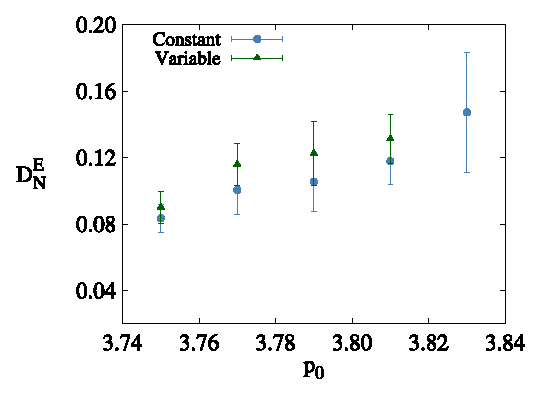
\includegraphics{fig9.eps}
% 	\caption{\label{EM_P0_D}Generalized distance to ultrametricity, for the normalized energy metric, $D^E_N$, as a function of $p_0$, for $N=1024$. These results were averaged over $10$ different systems with each being perturbed and re-minimized $100$ different times. The results represent the values measured using the constant $\varepsilon_{max}$ as in the main text, and a variable one that depends on $p_0$.}
% \end{figure}
%
% \subsection{Different perturbation protocols}
%
% To analyze the sensitivity to the perturbation protocol, we tested different approaches. Aside from the protocol presented in the main text we introduce two new ones, one based on Gaussian perturbations and another where some skeweness is added.
%
% In the Gaussian perturbation (G), we start by creating a perturbation vector $\overrightarrow{P}_{\varepsilon}=[X_0, X_1, X_2, X_3, ... , X_{2N-1}]$, where $N$ is the number of cells, $X_{2i}=\mathcal{N}(0,1)$ is the perturbation to cell $i$ along the $x$-axis and $X_{2i+1}=\mathcal{N}(0,1)$ is the one along the $y$-axis. Here, $\mathcal{N}(0,1)$ represents a normal distribution with mean $\mu=0$ and standard deviation $\sigma=1$. Then we subtract the global translation of the system after perturbation. Finally, we multiply the perturbation vector by $\varepsilon$, which is a uniformly distributed random variable between $0$ and $\varepsilon_{max}$. With this formulation, the norm of the perturbation vector will scale as $|\overrightarrow{P}_{\varepsilon}|=P_{\varepsilon}=\varepsilon\sqrt{2N}\sigma$.
%
% In the Skewed perturbation (S), we start by defining a perturbation vector $\overrightarrow{P}_{\varepsilon}=[X_0, X_1, X_2, X_3, ... , X_{2N-1}]$, where $X_{2i}=\mathcal{N}(0,1)+\mathcal{E}(0.5)$ is the perturbation to cell $i$ along the $x$-axis and $X_{2i+1}=\mathcal{N}(0,1)+\mathcal{E}(0.5)$ is the one along the $y$-axis. Here, $\mathcal{E}(0.5)$ represents a Poisson distribution with rate $\lambda=0.5$. Then we subtract the global translation of the system after perturbation. Finally, we multiply the perturbation vector by $\varepsilon$, which is a uniformly distributed random variable between $0$ and $\varepsilon_{max}$. By adding a Poisson distribution we are skewing the positive Gaussian tail. With this formulation, the norm of the perturbation vector will scale as $|\overrightarrow{P}_{\varepsilon}|=P_{\varepsilon}=\varepsilon\sqrt{2N(\sigma^2+1/\lambda^2)}$.
%
% In Fig.~\ref{EM_DP} is represented the generalized distance to ultrametricity, $D^E_N$, as a function of $p_0$, calculated using multiple perturbations to the same minimum. The maximum perturbation displacement was fixed at $\varepsilon_{max}=0.1\sqrt{N}$ for all protocols. We can observe that the different perturbations do not lead to different results and thus the range of distances found will only depend on the norm of the perturbation vector.
%
% \begin{figure}[t]
% 	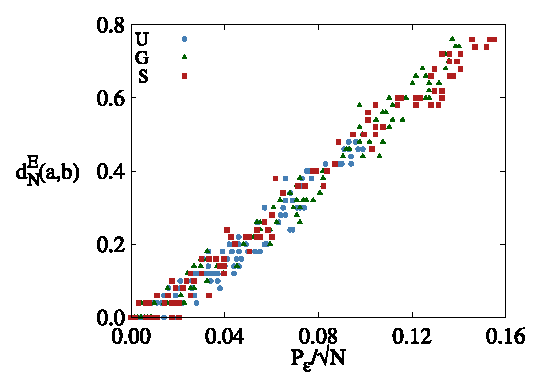
\includegraphics{fig10.eps}
% 	\caption{\label{EM_DP}Generalized distance to ultrametricity, $D^E_N$, as a function of $p_0$ for the different perturbations, using the normalized energy metric, $d^E_N(a,b)$. U represents the perturbation used in the main text. The size of the system is $N=1024$ and $\varepsilon_{max}=0.1\sqrt{N}$ for all. The individual parameters of the perturbations are summarized in the text.}
% \end{figure}
%
% \subsection{Estimation of the rigid to fluid transition point}
%
% To estimate the transition point from the rigid to a fluid tissue we use a technique based on recent work on the vertex model~\cite{Merkel2018}. We use the minimized configurations calculated in the main text and calculate the probability of finding a configuration with zero energy, $P[E=0]$, for different $p_0$ and $N$. Since we have less data for the different $p_0$ than in Ref.~\cite{Merkel2018}, we are not able to properly use the numerical integration proposed there and instead we fit our data to an hyperbolic tangent:
%
% \begin{equation}\label{tanh}
% 	P[E=0](p_0)=0.5\big[1-\text{tanh}\big(-\frac{p_0-a}{2b}\big)\big],
% \end{equation}
%
% \noindent where $a$ and $b$ are fitting parameters. Even though we do not expect that the actual function is Eq.~\eqref{tanh}, it serves as a good approximation for the $N$ explored here. By using this continuum function we are able to easily differentiate it and calculate the probability distribution of transition points, $P(p_0^*)=\text{d}_{p_0^*} P[E=0](p_0^*) $, from which we can extract the peak value corresponding to the probable transition point $p_0^*$ for a given $N$. Figure \ref{SM_P0} shows how $P[E=0](p_0)$ increases with $p_0$ and the corresponding fit given by Eq.~\eqref{tanh}, which is in good agreement. The right plot shows the derivative of Eq.~\eqref{tanh} as a function of $p_0^*$. We use the value corresponding to the peak of the distribution to estimate the transition points for the different $N$.
%
% \begin{figure*}[t]
% 	\includegraphics{fig11.eps}
% 	\caption{\label{SM_P0}On the left is plotted the probability of finding a configuration with zero energy, $P[E=0]$, as a function of $p_0$ for different $N$. These results were averaged over $1000$ samples. We also show a fit of Eq.~\eqref{SM_P0} to the data. On the right is the estimation of the transition point, $p_0^*$, which is calculated using the peak value of the probability distribution function of the transition points, $P(p_0^*)=\text{d}_{p_0^*}P[E=0](p_0^*)$.}
% \end{figure*}
%
% To estimate the transition point in the thermodynamic limit we check the best linear fit in a log-log plot, of the distance of the estimated $p_0^*$ for each $N$ (given by Fig.~\ref{SM_P0}) to the thermodynamic transition point $p_0^*(\infty)$, as a function of $1/N$. Figure \ref{SM_P0_2} shows the different curves for multiple $p_0^*(\infty)$ where we try to estimate the actual value for which the linear fit is best. We focus only on $N>1024$ and estimate that $p_0^*(\infty)=3.8022\pm 0.0001$. Although more simulations and a more appropriate estimation protocol should be used to properly quantify this value, our simple estimation falls close to the one reported in previous work~\cite{Sussman2018}.
%
% \begin{figure}[t]
% 	\includegraphics{fig12.eps}
% 	\caption{\label{SM_P0_2}Log-log plot of the absolute distance of the estimated transition pints for the different $N$ (from Fig.~\ref{SM_P0}) to the thermodynamic value, $p_0^*(\infty)$, as a function of $1/N$. We find $p_0^*(\infty)=3.8022\pm0.0001$ is the value which gives the best line fit for $N>1024$ and as such is our estimation of the transition point.}
% \end{figure}

% Create the reference section using BibTeX:
\bibliography{Glass}

\end{document}
